% SPDX-License-Identifier: CC0-1.0

\section{Arduino}


\begin{frame}{O Projeto Arduino}

	Surgiu em 2005 com base em outro projeto da época, chamado \Link[Wiring]{https://pt.wikipedia.org/wiki/Wiring}, cuja proposta era uma plataforma eletrônica aberta e fácil para iniciantes.

	\medskip
	Características:
	\begin{itemize}
		\item Baixo custo
		\item Multiplataforma
		\item Ambiente de desenvolvimento simples e intuitivo
		\item Hardware/software \textit{open source} extensíveis
	\end{itemize}

\end{frame}


\subsection{Hardware: Mega 2560}


\begin{frame}[b]{\insertsubsection}

	Nossa placa usa o microcontrolador ATmega2560
	\begin{description}
		\item[7 V -- 12 V] Tensão de alimentação recomendada
		\item[5 V] Tensão de operação
		\item[16 MHz] Frequência de operação (\textit{clock rate})
		\item[256 KB] Memória flash
		\item[8 KB] SRAM
		\item[4 KB] EEPROM
		\item[54] Pinos digitais (\Highlight{15} com saída PWM)
		\item[16] Pinos com conversor analógico-digital
		\item[20 mA] Limite de corrente por pino
	\end{description}

	\vfill
	Leitura interessante: \Link[MPU vs.\@ MCU]{https://semiengineering.com/mpu-vs-mcu}, \Link[Microcontrollers vs.\@ Microprocessors: What’s the difference?]{https://www.microcontrollertips.com/microcontrollers-vs-microprocessors-whats-difference}

\end{frame}


{ \definecolor{background}{named}{white}
\begin{frame}{\insertsubsection}

	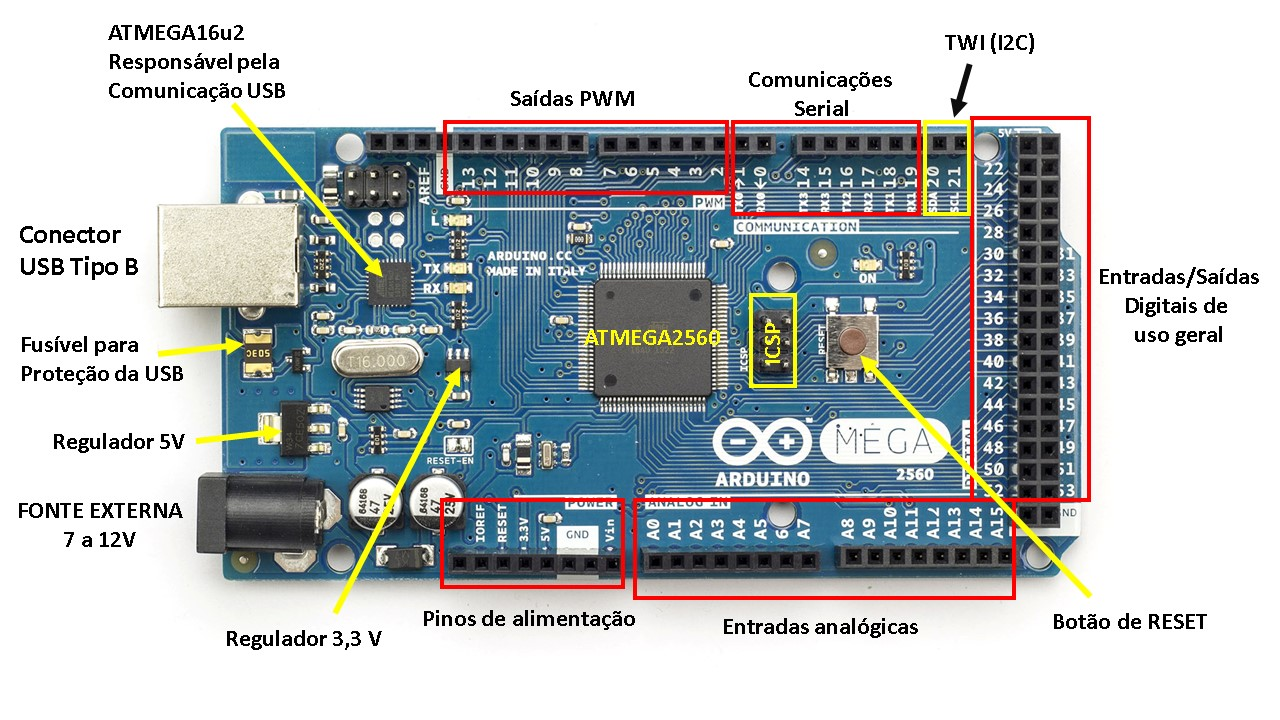
\includegraphics[width=\linewidth]{mega2560.jpg}

\end{frame}
}


\subsection{Software: IDE}


\begin{frame}[b]{\insertsubsection}

	O ambiente de desenvolvimento que usaremos pode ser baixado em
	\begin{center}
		\Link[\texttt{arduino.cc/en/main/software}]{https://www.arduino.cc/en/main/software}
	\end{center}

	\vfill
	No entanto, há outras ferramentas, como
	\begin{enumerate}
		\item \Link[Arduino Create]{https://create.arduino.cc}
		\item \Link[Tinkercad Circuits]{https://www.tinkercad.com/learn/circuits}
		\item \Link[XOD]{https://xod.io}
		\item \Link[Arduino Pro IDE]{https://github.com/arduino/arduino-pro-ide/releases/latest}
		\item \Link[pyFirmata]{https://pypi.org/project/pyFirmata}
	\end{enumerate}

\end{frame}


{ \definecolor{background}{named}{white}

\begin{frame}{\insertsubsection}

	\begin{columns}[onlytextwidth]
	\column[c]{0.55\linewidth}
		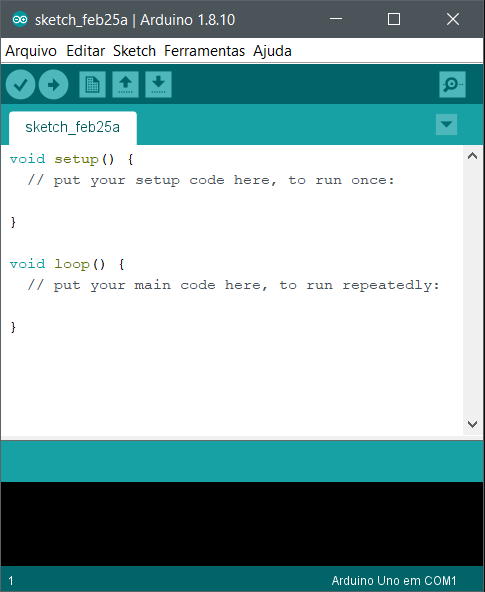
\includegraphics[height=0.85\textheight]{ideMainScreen.png}
	\column[c]{0.45\linewidth}
		\begin{tabular}{p{2ex}p{0.77\linewidth}}
			\multirow{2}{*}{
\includegraphics[height=3ex]{ideToolbarVerify.png}} & \textcolor{ArduinoTeal}{Verificar} \\
			\smallskip & {\small Verifica erros de compilação no seu código.} \\
			\multirow{2}{*}{
\includegraphics[height=3ex]{ideToolbarUpload.png}} & \textcolor{ArduinoTeal}{Carregar} \\
			\smallskip & {\small Compila e carrega seu código para a placa.} \\
			\multirow{2}{*}{
\includegraphics[height=3ex]{ideToolbarNew.png}} & \textcolor{ArduinoTeal}{Novo} \\
			\smallskip & {\small Cria um novo \textit{sketch}.} \\
			\multirow{2}{*}{
\includegraphics[height=3ex]{ideToolbarOpen.png}} & \textcolor{ArduinoTeal}{Abrir} \\
			\smallskip & {\small Abre um \textit{sketch}.} \\
			\multirow{2}{*}{
\includegraphics[height=3ex]{ideToolbarSave.png}} & \textcolor{ArduinoTeal}{Salvar} \\
			\smallskip & {\small Salva seu \textit{sketch}.} \\
			\multirow{2}{*}{
\includegraphics[height=3ex]{ideToolbarSerialMonitor.png}} & \textcolor{ArduinoTeal}{Monitor Serial} \\
			\smallskip & {\small É um Terminal para interação com a placa.} \\
		\end{tabular}
	\end{columns}

\end{frame}


\begin{frame}[focus]

	Pluguem suas placas.

\end{frame}


\begin{frame}{\insertsubsection}

	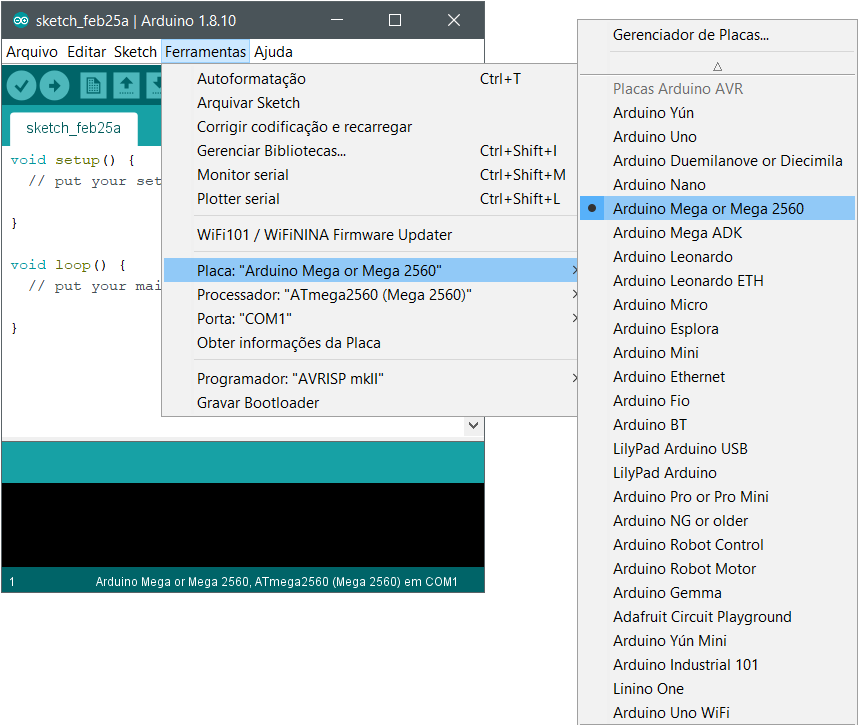
\includegraphics[height=0.85\textheight,trim={0 28mm 0 0}]{ideMenuToolsBoard.png}

\end{frame}


\begin{frame}{\insertsubsection}

	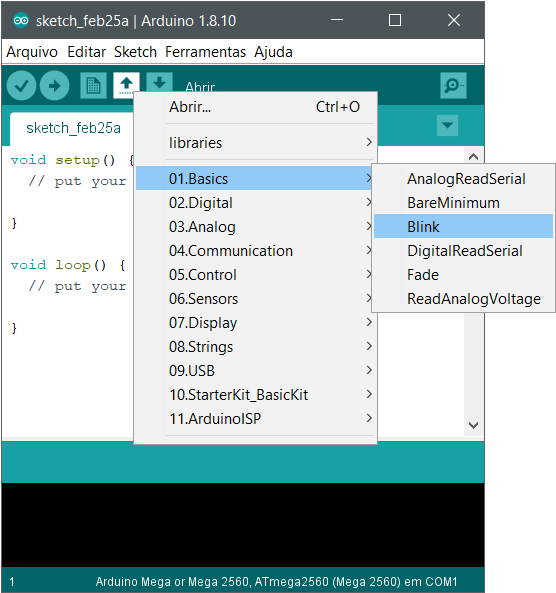
\includegraphics[height=0.85\textheight]{ideMenuExamplesBlink.png}

\end{frame}


\begin{frame}{\insertsubsection}

	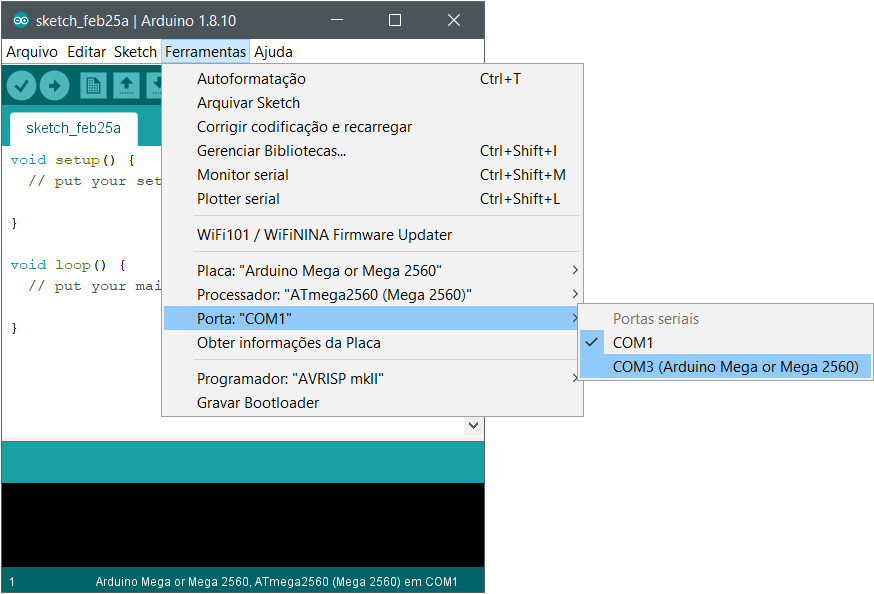
\includegraphics[height=0.85\textheight]{ideMenuToolsPort.png}

\end{frame}

} % Fim do \definecolor
